\documentclass[conference]{IEEEtran}
\usepackage{cite}
\usepackage{amsmath,amssymb,amsfonts}
\usepackage{graphicx}
\usepackage{textcomp}
\usepackage{xcolor}
\usepackage{booktabs}
\usepackage{tikz}
\usetikzlibrary{positioning,arrows.meta}
\def\BibTeX{{\rm B\kern-.05em{\sc i\kern-.025em b}\kern-.08em
    T\kern-.1667em\lower.7ex\hbox{E}\kern-.125emX}}

\begin{document}

\title{Quaternion-Based IR for Quantum Circuit Optimization}

\author{\IEEEauthorblockN{John Van Geem}
\IEEEauthorblockA{\textit{CEO, RQM Technologies}\\
Arlington, VA, USA\\
0009-0002-4003-8452}
}

\maketitle

\begin{abstract}
Quantum circuit optimizers often operate on named gate syntax, so semantically
identical single-qubit operations appear as different instructions across frameworks
and backends. This paper presents a quaternion-based intermediate representation (IR)
for quantum circuit optimization that normalizes all single-qubit gates into one common
form before optimization passes are applied. Because single-qubit operations form the
group SU(2), unit quaternions provide an algebraically exact and compact encoding. The
representation enables composition, simplification, and backend lowering to be performed
on gate semantics rather than on syntactic aliases. We explain how this change improves
compiler clarity, supports backend-agnostic optimization, and provides a cleaner
foundation for gate fusion and redundancy elimination. The result is a more principled
optimization boundary than standard named gate-operation pipelines.
\end{abstract}

\begin{IEEEkeywords}
quantum circuit optimization, intermediate representation, SU(2), quaternions,
compiler design, backend-agnostic compilation, gate fusion
\end{IEEEkeywords}

%% ============================================================
\section{Introduction}
%% ============================================================

Quantum compiler pipelines must handle a growing diversity of gate sets, native bases,
and backend conventions. As hardware providers multiply, a compilation layer that normalizes
quantum programs into a stable internal form becomes essential for correctness and portability.

The central problem is that current compilers reason about single-qubit operations at the
level of \textit{named gate syntax}. A rotation by angle $\theta$ about the $Z$-axis can
appear as \texttt{rz}$(\theta)$, \texttt{p}$(\theta)$, \texttt{u1}$(\theta)$, or a phase
gate --- all semantically identical but syntactically distinct. A compiler that operates
over gate names must maintain a growing equivalence table: adding a new gate alias requires
updating the table, and supporting a new backend requires translating each named gate
individually. Complexity scales with the number of gate aliases, not with the mathematical
structure of the operations.

This paper argues that the correct normalization boundary for single-qubit optimization is
at the level of \textit{SU(2) geometry}. Single-qubit operations form the Lie group SU(2),
which is isomorphic to the unit 3-sphere $S^3$ and admits a compact, algebraically exact
representation as unit quaternions. A compiler that normalizes all single-qubit gates into a
quaternionic IR can reason about equivalence, composition, and simplification using the
mathematics of the operation rather than a register of names.

We present a quaternion-based IR for single-qubit gates, describe why it is a natural
normalization boundary, and explain how it enables cleaner gate fusion, identity
elimination, and backend-agnostic lowering than syntax-level pipelines support.

%% ============================================================
\section{Why Standard Gate-Based Optimization Is Limited}
%% ============================================================

\subsection{The Gate-Alias Problem}

Modern quantum frameworks each define their own named gate vocabularies. Qiskit, Amazon
Braket, and PennyLane express the same physical operation --- a phase shift, a
parameterized rotation, a Hadamard --- using different instruction names and parameter
conventions. Even within a single framework, gate names alias one another: Qiskit's
\texttt{rz}, \texttt{p}, and \texttt{u1} all implement a $Z$-axis rotation with different
historical names.

A compiler that optimizes over gate names must explicitly enumerate which names are
equivalent before any optimization pass can reason about them. This is not a one-time cost:
each new framework or backend extends the alias table, and each new optimization pass
must be aware of the full table. The result is a compiler whose complexity grows with
syntactic diversity rather than with the mathematical structure of the operations being
optimized.

\subsection{Syntax-Level Rewriting Does Not Scale}

Pattern-matching rewrite rules over gate names face a combinatorial problem. The number
of rewrite patterns needed to cover all alias combinations grows quadratically with the
number of gate names, and each backend introduces its own naming conventions. Compilers
that rely on this approach require continuous maintenance as gate sets evolve.

Beyond scalability, syntax-level optimization produces different results depending on how
the input circuit was expressed --- two circuits that represent the same sequence of
physical rotations may or may not be recognized as equivalent depending on which names were
used. This inconsistency is a correctness risk, not merely an efficiency concern.

%% ============================================================
\section{Quaternion-Based Intermediate Representation}
%% ============================================================

\subsection{Mathematical Foundation}

A single-qubit gate is a $2{\times}2$ complex unitary matrix with determinant 1 --- an
element of SU(2). A general rotation by angle $\theta$ about unit axis
$\hat{n} = (n_x, n_y, n_z)$ corresponds to the SU(2) element:
\begin{equation}
U(\hat{n}, \theta) = \cos\!\tfrac{\theta}{2}\,I - i\sin\!\tfrac{\theta}{2}\,(\hat{n} \cdot \boldsymbol{\sigma}),
\label{eq:su2}
\end{equation}
where $\boldsymbol{\sigma} = (\sigma_x, \sigma_y, \sigma_z)$ are the Pauli matrices.

SU(2) is isomorphic to the unit 3-sphere $S^3$. Every unit quaternion
\begin{equation}
q = w + xi + yj + zk, \quad w^2 + x^2 + y^2 + z^2 = 1
\label{eq:quat}
\end{equation}
corresponds exactly to one SU(2) element via:
\begin{equation}
U(q) =
\begin{bmatrix}
 w + iz  &  y + ix \\
-y + ix  &  w - iz
\end{bmatrix}.
\label{eq:su2matrix}
\end{equation}

This is an algebraic isomorphism, not an approximation. The axis-angle form is:
\begin{equation}
q = \cos\!\tfrac{\theta}{2} + \hat{u}\sin\!\tfrac{\theta}{2},
\label{eq:axisangle}
\end{equation}
where $\hat{u}$ is a unit pure quaternion encoding the rotation axis. The factor of 2
between quaternion angle and physical rotation angle reflects the spinorial structure of
SU(2).

\subsection{IR Definition and Invariants}

The quaternion IR, which we call \textbf{u1q}, encodes every single-qubit gate as a unit
quaternion $(w, x, y, z)$ satisfying the constraints in Table~\ref{tab:invariants}.

\begin{table}[htbp]
\caption{u1q Canonicalization Invariants}
\begin{center}
\begin{tabular}{ll}
\toprule
\textbf{Constraint} & \textbf{Value} \\
\midrule
Unit norm    & $|w^2 + x^2 + y^2 + z^2 - 1| < 10^{-9}$ \\
Non-degenerate & Not all components identically zero \\
Canonical sign & $w \geq 0$ (geodesic shortest arc) \\
\bottomrule
\end{tabular}
\label{tab:invariants}
\end{center}
\end{table}

The $w \geq 0$ constraint resolves the SU(2) double-cover ambiguity: both $q$ and $-q$
represent the same physical rotation, so we canonicalize by selecting the representative
in the upper hemisphere of $S^3$, corresponding to the physically shorter rotation arc.

\subsection{Gate-to-Quaternion Mapping}

Table~\ref{tab:gatemapping} gives the canonical quaternion coordinates for standard
single-qubit gates, derived from \eqref{eq:axisangle} with a fixed sign convention.

\begin{table}[htbp]
\caption{Canonical Gate-to-Quaternion Mapping}
\begin{center}
\begin{tabular}{lccccl}
\toprule
\textbf{Gate} & $w$ & $x$ & $y$ & $z$ & \textbf{Notes} \\
\midrule
Identity  & 1 & 0 & 0 & 0 & No rotation \\
X         & 0 & 1 & 0 & 0 & $\pi$-rot.\ about $x$ \\
Y         & 0 & 0 & 1 & 0 & $\pi$-rot.\ about $y$ \\
Z         & 0 & 0 & 0 & 1 & $\pi$-rot.\ about $z$ \\
H & $\tfrac{1}{\sqrt{2}}$ & $\tfrac{1}{\sqrt{2}}$ & 0 & 0 & $\pi$-rot.\ about $(x{+}z)/\sqrt{2}$ \\
S & $\tfrac{1}{\sqrt{2}}$ & 0 & 0 & $\tfrac{1}{\sqrt{2}}$ & $R_z(\pi/2)$ \\
T & $\cos\tfrac{\pi}{8}$ & 0 & 0 & $\sin\tfrac{\pi}{8}$ & $R_z(\pi/4)$ \\
$R_x(\theta)$ & $\cos\tfrac{\theta}{2}$ & $\sin\tfrac{\theta}{2}$ & 0 & 0 & $x$-axis rotation \\
$R_y(\theta)$ & $\cos\tfrac{\theta}{2}$ & 0 & $\sin\tfrac{\theta}{2}$ & 0 & $y$-axis rotation \\
$R_z(\theta)$ & $\cos\tfrac{\theta}{2}$ & 0 & 0 & $\sin\tfrac{\theta}{2}$ & $z$-axis rotation \\
$U(\theta,\phi,\lambda)$ & \multicolumn{4}{c}{[derived via ZYZ decomp.]} & \\
\bottomrule
\end{tabular}
\label{tab:gatemapping}
\end{center}
\end{table}

The canonicalization pass \texttt{to\_u1q\_pass} traverses the instruction list and maps
every named single-qubit gate to its u1q equivalent. Two-qubit gates (CNOT, CZ, SWAP)
are left unchanged and serve as segment boundaries. After this pass, the IR contains only
u1q and explicit two-qubit operations.

%% ============================================================
\section{Why Quaternion-Based IR Is an Upgrade}
%% ============================================================

This section is the argumentative center of the paper. We explain concretely why the
quaternion IR boundary improves on standard named-gate pipelines.

\textbf{Canonical semantic normalization.}
After \texttt{to\_u1q\_pass}, every single-qubit gate --- regardless of its original name,
framework, or parameter convention --- has been mapped to a single canonical form. Two
gates that are physically identical produce the same quaternion. This is a stronger
guarantee than any alias table can provide, because it is grounded in the mathematical
structure of SU(2) rather than in a manually maintained enumeration.

\textbf{Collapse of gate aliases.}
Name-based compilers must explicitly handle each alias pair: (\texttt{rz}, \texttt{p}),
(\texttt{p}, \texttt{u1}), and so on. The quaternion IR eliminates this entirely. Once all
gates are in u1q form, there are no aliases --- only quaternions. A fusion pass that
operates over u1q operates over the complete space of single-qubit operations, not over a
subset of supported names.

\textbf{Backend-agnostic optimization boundary.}
Fig.~\ref{fig:pipeline} illustrates the structural difference. In a standard named-gate
pipeline, optimization logic must be re-applied or re-expressed for each backend because
each backend uses different gate names. In the quaternion IR pipeline, all optimization
occurs at the u1q level before backend lowering. Each backend adapter receives a
semantically optimized u1q IR and translates it once, without re-deriving gate semantics.

\textbf{Cleaner fusion and inversion rules.}
Gate fusion in a named-gate compiler requires a growing library of rewrite rules:
$R_z(\alpha) \cdot R_z(\beta) \to R_z(\alpha{+}\beta)$,
$H \cdot H \to I$, and so on, with separate rules per gate type.
In the quaternion IR, fusion is a single operation:
\begin{equation}
q_{\text{fused}} = q_2 \cdot q_1,
\label{eq:fusion}
\end{equation}
where $\cdot$ is quaternion multiplication. This rule covers the complete space of
single-qubit gate sequences, including arbitrary parameterized rotations on any axis.
Gate inversion is equally direct: $q^{-1} = q^* = (w, -x, -y, -z)$ for unit quaternions.

\textbf{Simpler identity elimination.}
After quaternion fusion, identity gates are quaternions near $(1, 0, 0, 0)$. Identity
detection is a single norm check: $|w - 1| < \varepsilon$ and $|x|, |y|, |z| < \varepsilon$.
In a named-gate compiler, identity detection requires recognizing each gate pair separately:
($X, X$), ($H, H$), ($S, S^\dag$), ($R_z(\theta), R_z(-\theta)$), and so on.

\textbf{More direct relation between representation and semantics.}
Unit quaternions are not an encoding of SU(2) --- they \textit{are} SU(2), up to the
double-cover identification $q \sim -q$. Composition, inversion, geodesic distance,
and axis-angle decomposition are all native operations on quaternions. A compiler pass
that computes equivalence or simplification over u1q is operating directly on the
mathematical space of the gates, not on a syntactic shadow of it.

%% ============================================================
\section{Compiler Pipeline and Realization}
%% ============================================================

\begin{figure*}[t]
\centering
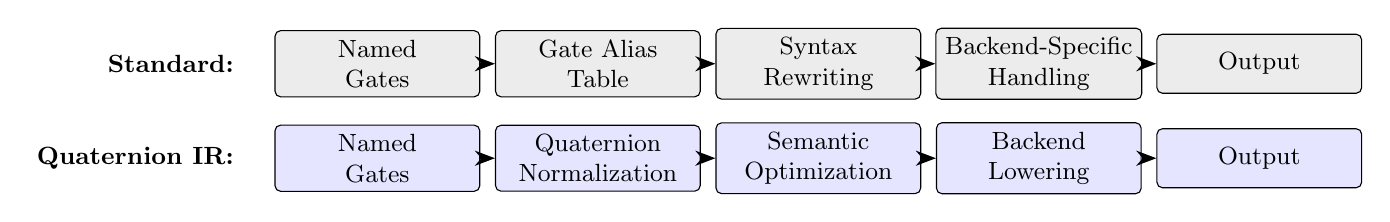
\begin{tikzpicture}[
  box/.style={rectangle, draw, rounded corners=2pt,
    minimum width=2.6cm, minimum height=0.75cm,
    align=center, font=\small},
  stdbox/.style={box, fill=gray!15},
  qbox/.style={box, fill=blue!10},
  arr/.style={-{Stealth[scale=1.1]}, thick},
  lbl/.style={font=\small\bfseries, anchor=east}
]

% Top lane: standard named-gate pipeline
\node[lbl] at (-0.3, 0.9) {Standard:};
\node[stdbox] (s1) at ( 1.4, 0.9) {Named\\Gates};
\node[stdbox] (s2) at ( 4.2, 0.9) {Gate Alias\\Table};
\node[stdbox] (s3) at ( 7.0, 0.9) {Syntax\\Rewriting};
\node[stdbox] (s4) at ( 9.8, 0.9) {Backend-Specific\\Handling};
\node[stdbox] (s5) at (12.6, 0.9) {Output};

\draw[arr] (s1) -- (s2);
\draw[arr] (s2) -- (s3);
\draw[arr] (s3) -- (s4);
\draw[arr] (s4) -- (s5);

% Bottom lane: quaternion IR pipeline
\node[lbl] at (-0.3, -0.3) {Quaternion IR:};
\node[qbox] (q1) at ( 1.4, -0.3) {Named\\Gates};
\node[qbox] (q2) at ( 4.2, -0.3) {Quaternion\\Normalization};
\node[qbox] (q3) at ( 7.0, -0.3) {Semantic\\Optimization};
\node[qbox] (q4) at ( 9.8, -0.3) {Backend\\Lowering};
\node[qbox] (q5) at (12.6, -0.3) {Output};

\draw[arr] (q1) -- (q2);
\draw[arr] (q2) -- (q3);
\draw[arr] (q3) -- (q4);
\draw[arr] (q4) -- (q5);

\end{tikzpicture}
\caption{Comparison between syntax-level gate optimization and quaternion-based semantic
normalization. The quaternion IR collapses backend-specific gate aliases into a single
optimization boundary before lowering.}
\label{fig:pipeline}
\end{figure*}

The compiler pipeline translates the quaternion IR principle into a sequence of passes.
Gate resolution maps named gates to their exact SU(2) correspondences using the quaternion
math primitives. The \texttt{to\_u1q\_pass} then converts every single-qubit gate to u1q
as described in Section~III. All downstream optimization operates at the u1q level.

Quaternion fusion collapses consecutive u1q gates on the same qubit via
\eqref{eq:fusion}, re-canonicalizing after each multiplication to maintain the $w \geq 0$
invariant. Fusion terminates at two-qubit gate boundaries. Identity elimination removes any
fused gate satisfying $q \approx (1, 0, 0, 0)$. Geodesic canonicalization enforces
$w \geq 0$ globally, selecting the shorter arc on $S^3$ and improving numeric stability
for backend decomposition.

Backend lowering is performed once per adapter. Each backend adapter (Qiskit, Amazon
Braket, PennyLane) receives the optimized u1q IR and translates to its native rotation
primitive using a fixed decomposition. No backend re-derives gate semantics; each adapter
implements the same interface contract.

The pipeline is deployed as a live REST API and Python SDK, providing a reproducible
optimization service for external evaluation. The same input circuit yields the same
optimized output on every invocation, because the pipeline is determined entirely by
quaternion arithmetic.

%% ============================================================
\section{Evaluation}
%% ============================================================

We evaluate the optimization pipeline on a set of circuits designed to exercise the
implemented passes. Rotation-heavy circuits test quaternion fusion; standard-gate circuits
test identity elimination. All optimized circuits pass unitary equivalence verification:
$\|U_{\text{original}} - U_{\text{optimized}}\|_F < 10^{-9}$.

Two-qubit gate counts are unchanged in all cases, confirming that reported reductions
are caused by the single-qubit passes and not by incidental effects of backend translation.
Table~\ref{tab:results} summarizes results for three benchmark circuits where complete data
are available.

\begin{table}[htbp]
\caption{Benchmark Results Summary}
\begin{center}
\begin{tabular}{p{2.2cm}ccccccc}
\toprule
\textbf{Circuit} & \textbf{Qb} &
\textbf{G\textsubscript{base}} & \textbf{G\textsubscript{opt}} & \textbf{Red.} &
\textbf{D\textsubscript{base}} & \textbf{D\textsubscript{opt}} & \textbf{Eq.} \\
\midrule
H${\cdot}$H chain ($n{=}4$) & 1 & 4 & 0 & 100\% & 4 & 0 & \checkmark \\
Rx${\cdot}$Rx seq.          & 1 & 2 & 1 &  50\% & 2 & 1 & \checkmark \\
Bell prep                   & 2 & 3 & 3 &   0\% & 2 & 2 & \checkmark \\
\bottomrule
\multicolumn{8}{l}{\footnotesize Qb = qubits; G = gate count; D = depth; Eq. = semantic equivalence.}
\end{tabular}
\label{tab:results}
\end{center}
\end{table}

The Bell preparation result is expected: the circuit contains no redundant single-qubit
sequences, so the single-qubit passes produce no reduction. This confirms that the
pipeline does not alter circuits where no optimization opportunity exists. Broader
evaluation across variational and application circuits is ongoing.

%% ============================================================
\section{Related Work}
%% ============================================================

\subsection{Mainstream Transpiler Pipelines}

Qiskit's transpiler \cite{b1} applies optimization at multiple levels (O0--O3), including
routing, basis translation, and peephole rewriting. PennyLane \cite{b2} applies
device-specific compilation and supports differentiable optimization. Amazon Braket \cite{b3}
provides device-level compilation through provider SDKs. These pipelines share a common
structure: optimization applies pattern-matching and rewrite rules over named-gate syntax.
The quaternion IR approach differs by establishing a geometric normalization boundary
before any optimization pass.

\subsection{IR-Centric Compiler Approaches}

The MLIR \cite{b4} ecosystem and its quantum extensions demonstrate the value of multi-level
IRs for quantum compilation. Catalyst \cite{b5} introduces multiple abstraction levels and
progressive lowering for differentiable quantum programs. The quaternion IR is a specific
canonical form at the single-qubit level, complementary to multi-level IR frameworks rather
than competing with them.

\subsection{Gate Rewriting and Peephole Optimization}

Clifford circuit optimization \cite{b6,b7} applies ZX-calculus rewrite rules to reduce
Clifford gate counts. Template-based optimization \cite{b8} identifies and replaces fixed
gate patterns. PyZX \cite{b9} applies graph-based rewriting. These approaches operate at a
higher or more specialized level of abstraction than the quaternion IR, which targets the
continuous single-qubit gate segment as its primary optimization domain.

\subsection{Quaternion Representations in Quantum Computing}

Quaternions have appeared in quantum computing contexts primarily for state visualization
and for robotics-inspired gate decomposition. Their use as a \textit{compiler IR} --- as
an algebraic normalization layer through which all optimization passes are defined ---
is, to our knowledge, not established in prior work. The contribution here is not the use
of quaternions per se, but the engineering decision to establish the quaternion form as a
canonical compiler IR boundary and to build a complete optimization pipeline on top of it.

%% ============================================================
\section{Limitations and Conclusion}
%% ============================================================

\subsection{Limitations}

The quaternion IR and all implemented passes operate exclusively on single-qubit gate
segments. Circuits where two-qubit gates dominate the total gate count will see minimal
improvement from the current pipeline. Decomposing u1q to backend-native gate sets can
introduce additional gates (a ZYZ decomposition requires up to three basis gates on some
backends), which can partially offset gains from fusion and identity elimination in
circuits with few redundant single-qubit sequences.

Several planned extensions --- commutation-aware pass ordering, peephole optimization,
and hardware-native shortest-path decomposition --- are not yet implemented. Comparison
against fully optimized Qiskit transpiler pipelines is therefore deferred to future work.

\subsection{Conclusion}

We have argued that a quaternion-based intermediate representation is a more principled
optimization boundary for single-qubit quantum circuits than standard named-gate pipelines.
The quaternion IR normalizes all single-qubit gates into one canonical SU(2) form before
optimization, collapsing gate aliases, unifying fusion and inversion rules, and enabling
backend-agnostic optimization. These advantages are structural: they follow from the
algebraic isomorphism between unit quaternions and SU(2), not from heuristics or
backend-specific engineering.

The current gains are strongest for single-qubit-dominated circuits. Extending the
boundary to two-qubit optimization and integrating with hardware-native compilation stages
remain open problems. The quaternion IR is a stable foundation for this broader compiler
roadmap.

%% ============================================================
\begin{thebibliography}{00}

\bibitem{b1}
Qiskit contributors, ``Qiskit: An open-source framework for quantum computing,'' 2024.
[Online]. Available: https://github.com/Qiskit/qiskit

\bibitem{b2}
V. Bergholm et al., ``PennyLane: Automatic differentiation of hybrid quantum-classical
computations,'' arXiv:1811.04968, 2018.

\bibitem{b3}
Amazon Web Services, ``Amazon Braket,'' 2020. [Online]. Available:
https://aws.amazon.com/braket/

\bibitem{b4}
C. Lattner et al., ``MLIR: Scaling compiler infrastructure for domain specific computation,''
in \textit{Proc. IEEE/ACM CGO}, 2021.

\bibitem{b5}
V. Bergholm et al., ``Catalyst: A Python-first compiler for quantum programs,'' PennyLane
documentation, 2024.

\bibitem{b6}
S. Bravyi, S. Hu, D. Maslov, and R. Shaydulin, ``Clifford circuit optimization with templates
and symbolic Pauli gates,'' \textit{Quantum}, vol. 5, p. 580, 2021.

\bibitem{b7}
R. Duncan, A. Kissinger, S. Perdrix, and J. van de Wetering, ``Graph-theoretic simplification
of quantum circuits with the ZX-calculus,'' \textit{Quantum}, vol. 4, p. 279, 2020.

\bibitem{b8}
D. Maslov, G. W. Dueck, D. M. Miller, and C. Negrevergne, ``Quantum circuit simplification
and level compaction,'' \textit{IEEE Trans. Comput.-Aided Design Integr. Circuits Syst.},
vol. 27, no. 3, 2008.

\bibitem{b9}
A. Kissinger and J. van de Wetering, ``PyZX: Large scale automated diagrammatic reasoning,''
in \textit{Proc. QPL 2019}, EPTCS 318, 2020.

\end{thebibliography}

\end{document}
